Po zakończeniu pobierania obrazu instalatora należy nagrać go na zewnętrzny nośnik i uruchomić komputer z tego nośnika. Najlepszym rozwiązaniem jest użycie klucza usb (pendriva), gdyż obrazy instalacyjne Ubuntu są zbyt duże aby zmiejścić się na krążkach CD. Jednak nie wszystkie komputery potrafią startować z klucza USB. Jeżeli twój komputer nie ma takiej właściwości, będziesz musiał użyć płyty DVD lub karty (micro)SD.
\subsubsection{System Windows, nagrywanie na pendriva}
\begin{wrapfigure}[3]{r}{0.5\textwidth}
		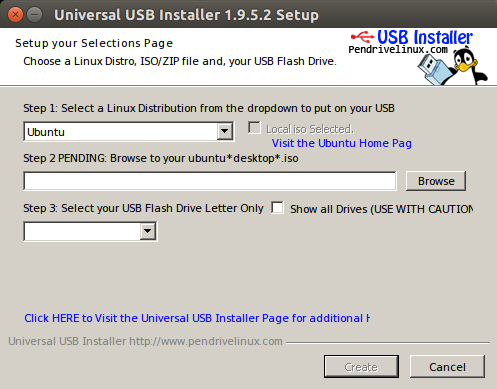
\includegraphics[width=\linewidth]{images/instalacja_nagrywanie_obrazu.png}
\end{wrapfigure}
\noindent Jeżeli chcesz użyć pendriva jako nośnika instalacyjnego to upewnij się iż ma on przynajmniej 1 gigabajt pojemności. W przeciwnym wypadku instalator nie zmiejści na nim. Jeżeli masz już przygotowany pendrive, wykonaj co następuje:
\begin{enumerate}
%TODO dla tej listy użyć włąsnych znaczników (label) przypominających te użyte na obrazkach.
\item Pobierz program \href{http://www.pendrivelinux.com/downloads/Universal-USB-Installer/Universal-USB-Installer-1.9.5.2.exe}{Universal USB Installer}.
\item Uruchom pobrany plik.
\item Zaakecptuj umowę licencyjną.
\item Podłącz do komputera pendrive, który ma użyty jako nośnik.
\item Z tej listy wybierz Ubuntu.
\item Kliknij na przycisk Browse i wskaż pobrany wcześniej obraz instalatora Ubuntu.
\item Z tej listy wybierz wczesniej podłączony pendrive.\\
\textbf{UWAGA: Wszystkie dane na nim zostaną skasowane!}
\item Kliknij przycisk CREATE.
\item Poczekaj na zakończenie operacji.
\end{enumerate}
\clearpage
\subsubsection{System Windows 7 / 8, nagrywanie na płytę DVD}
%TODO zweryfikować, czy windows 8 też to ma
\begin{wrapfigure}[3]{r}{0.5\textwidth}
		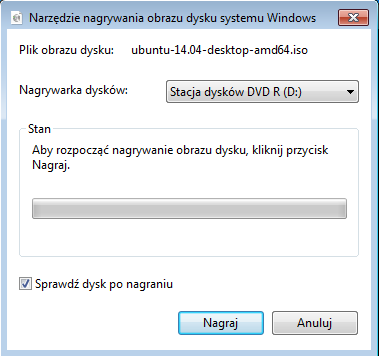
\includegraphics[width=\linewidth]{images/instalacja_nagrywanie_obrazu_DVD.png}
\end{wrapfigure}
Systemy operacyjne Windows 7 i 8 mają wbudowane narzędzie do wypalania plików .iso na płytach. Kliknij prawym przyciskiem myszy na pobrany obraz instalatora Ubuntu, wybierz opcję "Otwórz w" a następnie "Windows Disc Image Burner".
\begin{enumerate}
%TODO dla tej listy użyć włąsnych znaczników (label) przypominających te użyte na obrazkach.
%TODO jak to się po polsku nazywa?
\item Z tej listy wybierz swoją nagrywarkę.
\item Włóż czystą płytę DVD na wybranego napędu.
\item Upewnij się, że zaznaczone jest pole "Zweryfikuj dysk po nagraniu"
\item Kliknij na przycisk \textbf{Nagraj}
\end{enumerate}
\clearpage
\subsubsection{System Windows XP i inne starsze wersje, nagrywanie na płytę DVD}
\begin{wrapfigure}{R}{0.5\linewidth}
		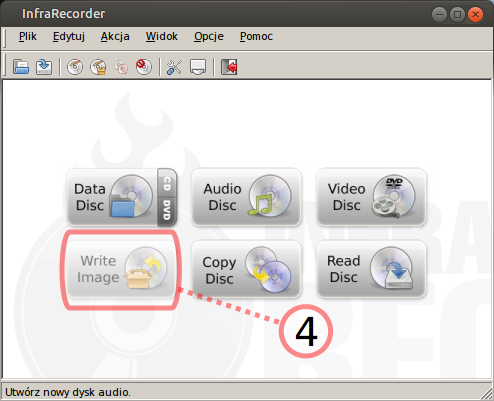
\includegraphics[width=\linewidth]{images/instalacja_nagrywanie_obrazu_DVD_winXP.png}
\end{wrapfigure}
Starsze wersje systemu Windows nie mają wbudowanej możliwości nagrywania płyt DVD. Potrzebne będzie do tego osobne narzędzie, program służący do wypalania płyt. Obsługa tych programów jest bardzo podobna: należy wybrać opcję \emph{Nagrywanie obrazu na płytę}. Koniecznie nagrywaj z wykorzystaniem tej opcji, gdyż inne (np.\emph{Nagrywanie płyty z danymi} lub \emph{Tworzenie kopi zapasowej}) utworzy dysk, którego twój komputer nie będzie potem wstanie uruchomić. Dla przykładu posłużymy się programem Infra Recorder.

\begin{enumerate}
\item Pobierz i zainstaluj program \href{http://infrarecorder.org/?page_id=5}{Infra Recorder}.
\item Uruchom nowozainstalowany program.
\item Włóż czystą płytę DVD do nagrywarki.
\item W programie Infra Recorder wybierz opcję \textbf{Write Image}.
\item Wybierz pobrany wcześniej obraz instalatora Ubuntu.
\item Kliknij na przycisk \textbf{OK}.
\end{enumerate}











